\section{Verification}
\label{section:verification}

\newcommand{\BX}{BX}

In this section we explore a specific approach to verifying BX. The approach we present is intended to be pragmatic, meant to be used with existing MDE tools and technologies. As such we do not consider issues such as soundness or completeness, though the mechanisms are present to prove conjectures related to these properties if so desired.

\BX\ are challenging to implement on account of the inherent complexity that they must encode. Model transformation languages supporting them often do so with conditions: some require that \BX\ are bijective (e.g.\ BOTL \cite{Braun-Marschall03a}), whereas others require users to work with specific formalisms such as triple graph grammars (e.g.\ MOFLON \cite{AKRS06a}).  Many modern transformation languages do not provide any support for \BX\ (e.g.\ ATL \cite{JABK08a}), meaning that users must express them as two unidirectional transformations. While this seems a practical workaround, the two transformations may diverge over time -- that is, there are no constructive guarantees that the two unidirectional transformations maintain the consistency relationship between the models being manipulated.
	
A trade-off between the benefits (but complexity) of pure \BX\ languages and the practicality (but possible incoherence) of unidirectional transformations can be achieved in Epsilon, a platform of interoperable and executable model management languages. Epsilon has languages supporting the specification of unidirectional transformations in either a rule-based (ETL), update-in-place (EWL), or operational (EOL) \cite{Paige-KRDP09a} style. Furthermore, it provides an inter-model consistency language (EVL \cite{Kolovos-Paige-Polack09a}) that can be used to express and evaluate constraints between models. With these languages, \BX\ can be ``faked'' by: (1) defining pairs of unidirectional transformations for separately updating the source and target models; and (2) defining inter-model constraints in EVL, the violation of which will trigger appropriate transformations to restore consistency.
	
Although this process gives us a means of checking consistency and automatically triggering a transformation to restore it, we lack the important guarantee that \BX\ give us: the compatibility of the transformations. It might be the case that after the execution of one transformation, the other does not actually restore consistency, leading to further EVL violations. Thus, how do we check for, and maintain, compatibility? 
	
We aim to obtain the guarantees of \BX\ without
the need for \BX\ languages. Instead, we can use \emph{rigorous} proof
techniques to verify that faked \BX\ are consistency preserving, and thus
indistinguishable to users from true \BX. To this end, we propose to apply
techniques from graph transformation verification. Given a faked \BX\ in
Epsilon, we will model the unidirectional transformations as graph
transformation rules, and EVL constraints as nested graph conditions
\cite{Habel-Pennemann09a}. Then, by leveraging graph transformation proof
calculi \cite{Habel-Pennemann-Rensink06a,Poskitt13a,Poskitt-Plump12a} in a
weakest precondition style, we aim to automatically prove compatibility of the
unidirectional transformations with respect to the EVL
constraints. 

\subsection{Illustration}
To illustrate the idea, consider yet again the OO to RDBMS problem. Class diagram models conform to a simple language describing familiar object-oriented concepts, whereas relational database models conform to a language describing how databases are constructed. Consistency is defined in terms of a correspondence between the data in the models, e.g.\ every table $n$ corresponds to a class $n$, and every column $m$ corresponds to an attribute $m$. Figure~\ref{fig:cd2rdbm_example} contains two simple models that are consistent in this sense (we omit the metamodels, but they are obvious).	

\begin{figure}[htbp]
\centering{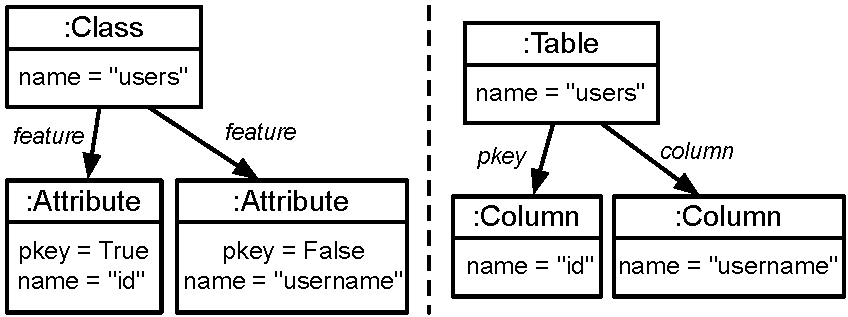
\includegraphics[width=0.6\textwidth]{cd2rdbm-ex.pdf}}
\caption{Two consistent OO and RDBMS models}
\label{fig:cd2rdbm_example}
\end{figure}

%	\begin{wrapfigure}[9]{r}{0.6\textwidth}
%		\centering
%			\vspace{-22pt}
%			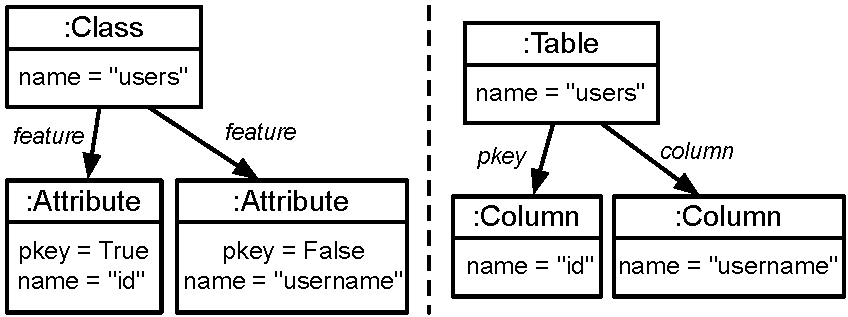
\includegraphics[width=0.6\textwidth]{cd2rdbm-ex.pdf}
%		\vspace{-21pt}\caption{Two consistent CD and RDB models}\label{fig:cd2rdbm_example}
%	\end{wrapfigure}
	
	Users of the models should be able to create new classes (or tables) whilst maintaining inter-model consistency. Upon the creation of a new class (resp.\ table), a table (resp.\ class) should be created with the same name to restore consistency. We can implement such a simple \BX\ in Epsilon with a pair of unidirectional transformations (one for updating the class diagram model, one for updating the relational database) and a set of EVL constraints. For the former, we can use the Epsilon Wizard Language (EWL) to define a pair of update-in-place transformations, $\tt AddClass$ and $\tt AddTable$ (for simplicity, here we assume the new class/table name $\tt newName$ to be pre-determined and unique, but Epsilon does support the capturing and sharing of such data between wizards).
	
%\vspace{-15pt}
%\begin{center}
%	\begin{minipage}[t]{0.475\textwidth}
	\begin{lstlisting}[language=java]
wizard AddClass {
 do {
   var c: new Class;
   c.name = newName;
   self.Class.all.first().contents.add(c);
 }}
 \end{lstlisting}
%	\end{minipage}
	\hspace{7pt}
%	\begin{minipage}[t]{0.475\textwidth}
	\begin{lstlisting}[language=java]
wizard AddTable {
 do {
   var table: new Table;
   table.name = newName;
   self.Table.all.first().contents.add(table);
 }}
	\end{lstlisting}
%	\end{minipage}
%\end{center}
%
%\vspace{-8pt}%

Using the Epsilon Validation Language (EVL), we express inter-model consistency: that for every class $n$, there exists a table named $n$ (and vice versa). If one of the constraints is violated, Epsilon can automatically trigger the relevant transformation to attempt to restore consistency. For example, after executing the transformation $\tt AddClass$, the constraint $\tt TableExists$ will be violated, indicating that the transformation $\tt AddTable$ should be executed to restore consistency.
	
%	\vspace{-15pt}\begin{center}
%		\begin{minipage}[t]{0.475\textwidth}
		\begin{lstlisting}[language=java]
context OO!Class {
 constraint TableExists {
   check : DB!Table.all.select(t|t.name = self.name).size() > 0
}}	
		 \end{lstlisting}
%		\end{minipage}
		\hspace{7pt}
%		\begin{minipage}[t]{0.475\textwidth}
		\begin{lstlisting}[language=java]
context DB!Table {
 constraint ClassExists {
   check : OO!Class.all.select(c|c.name = self.name).size() > 0
}}
		\end{lstlisting}
%		\end{minipage}
%	\end{center}	
%\vspace{-8pt}%

This example of a \BX, ``faked'' in Epsilon, is a simple one chosen to illustrate the concepts. Even what appears to be a simple \BX can lead to more interesting (i.e.\ less symmetric) \BX, e.g.\ manipulating inheritance in the class model.

\subsection{Checking Compatibility}
A critical difference between the ``faked'' \BX\ in the previous section and a true \BX\ is the absence of guarantees about the compatibility of the transformations: upon the violation of $\tt TableExists$, for example, does the execution of $\tt AddTable$ actually restore consistency? For this simple example, a manual inspection will quickly confirm that the transformations are indeed compatible. But what about more intricate \BX? And what about \BX\ that evolve and change over time? For the Epsilon-based approach to be a convincing alternative to a \BX\ language, it is imperative that the compatibility of the transformations can be checked, and that this can be done in a simple and automatic way. To this end, we propose to leverage and adapt some recent developments in the verification of graph transformations.
	
	Graph transformation is a computation abstraction: the state of a computation is represented as a graph, and the computational steps as applications of rules (i.e.\ akin to string rewriting in Chomsky grammars, but lifted to graphs). Modelling a problem using graph transformation brings an immediate benefit in visualisation, but also an important one in terms of semantics: the abstraction has a well-developed algebraic theory that can be used for formal reasoning. This has been exploited to facilitate the verification of graph transformation systems, i.e.\ calculi for systematically proving specifications about graph properties before and after any execution of some given rules. Furthermore, such calculi have been generalised to graph programs \cite{Plump12a}, which augment the abstraction with expressions over labels and familiar control constructs (e.g.\ sequential composition, branching) for restricting the application of rules. In particular, we look to exploit work by Poskitt and Plump who developed proof calculi for graph programs, separately addressing reasoning about programs and properties involving attribute manipulation \cite{Poskitt13a,Poskitt-Plump12a}, as well as reasoning about non-local structural properties \cite{Poskitt-Plump14a}.

Our example \BX\ for the OO2RDBMS problem is easily translated into graph programs and nested conditions, as given in Figure \ref{fig:ex-program-constraints}. The programs $P_S,P_T$ are the individual rules creating respectively a class or table node labelled $\tt newName$ (here, $\emptyset$ denotes the empty graph, indicating that the rules can be applied without first matching any structure, i.e.\ unconditionally). The nested condition $evl$, given on the right, expresses that for every class (resp.\ table) node, there is a table (resp.\ class) node with the same name (we do not define here a formal interpretation, but note that $\tt x,y$ are variables, and that the numbers indicate when nodes are the same down the nesting of the formula). Were the weakest liberal preconditions to be constructed, we would find:
	\[ \text{Wlp}(P_S;P_T,evl) \equiv \text{Wlp}(P_T;P_S,evl) \equiv evl. \]
	
	\noindent Since $evl \Rightarrow evl$ is clearly valid, both $\{evl\}\ P_S;\ P_T\ \{evl\}$ and $\{evl\}\ P_T;\ P_S\ \{evl\}$ must hold, and---assuming correctness of the abstractions---the original EWL transformations are therefore compatible with respect to the EVL constraints.
	
	\begin{figure}[htb]
\vspace*{-10pt}
		\centering
		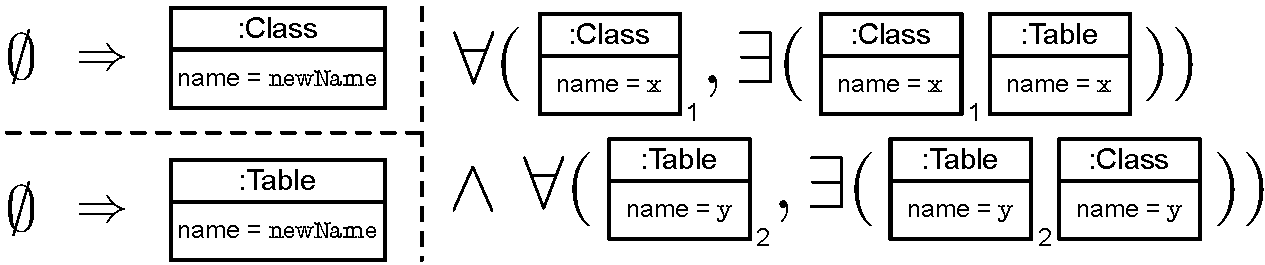
\includegraphics[width=0.8\textwidth]{ex-program-constraints.pdf}
		\caption{Our CD2RDBM \BX\ expressed as graph transformation rules and a nested condition}
\vspace*{-20pt}
		\label{fig:ex-program-constraints}
	\end{figure}

A key challenge with an approach such as this is what to do when the verification step fails, i.e., the implication above does not hold. We are exploring the use of the GROOVE tool to generate counterexamples when verification fails, via exploring executions of the graph transformation rules.
